%!TEX root = ComputerScienceOne.tex

%%Chapter: Searching & Sorting

Searching and sorting are two fundamental operations when dealing
with collections of data.  Both operations are not only important in
and of themselves, but they also form the basis of many other algorithms
and operations.  These operations are so essential that a wide variety
of algorithms and techniques have been developed to solve them, each
with their own advantages and disadvantages.  This variety provides
a good framework from which to study the relative efficiency and complexity
of algorithms through algorithm analysis.

\section{Searching}

Searching is a very basic operation.  Given a collection of data, we
wish to find a particular element or elements that match a certain 
criteria.  More formally, we have the following.

\begin{problem}[Searching]
\label{problem:searching}
~\\
\textbf{Given:} a collection of elements, $A =\{a_1, a_2, \ldots, a_n\}$ 
and a \emph{key} element $e_k$\\
\textbf{Output:} The element $a_i$ in $A$ such that $a_i = e_k$
\end{problem}

The ``equality'' or comparison in this problem statement is not explicitly 
specified.  In 
fact, this is a very general, abstract statement of the basic search 
problem.  We didn't specify that the ``collection'' was an array, a list, 
a set, or any other particular data structure.  Nor did we specify what
type of elements were in the collection.  They could be numbers, they
could be strings, they could be objects.  

There are many variations of this general search problem that we could
consider.  For example, we could generalize it to find the ``first''
or ``last'' such element if our collection is ordered.  We could find
\emph{all} elements that match our criteria.  Some basic operations that 
we've already considered such as finding the minimum or maximum
(\emph{extremal} elements), or median element are variations on this search 
problem.

When designing a solution to any of these variations additional 
considerations must be made.  We may wish our search to be index-based 
(that is, output the index $i$ rather than the element $a_i$).  We
may need to think about how to handle \emph{unsuccessful} searches 
(return \mintinline{text}{null}?  A special flag value?  Throw an
exception?, etc.).

When implementing a solution in a programming language, we of course
will need to be more specific about the type of collection being
searched, the type of elements in the collection, etc.  However, we
will still want to keep our solution as general as possible.  As we'll 
see, most programming languages facilitate some sort of \emph{generic}
programming so that we do not need to reimplement the solution for
\emph{each} type of collection or for \emph{each} type of variable.  
Instead, we can write one solution, then \emph{configure} it to allow
for comparisons of any type of variable (numeric, string, object, etc.).

\subsection{Linear Search}
\index{search!linear search}
\index{linear search}

The first solution that we'll look at is the \emph{linear search}
algorithm (also known as sequential search).  This is a basic, 
straightforward solution to the search problem that works by simply
iterating through each element $a_i$, testing for equality, and
outputting the first element that matches the criteria.  The
pseudocode is presented as Algorithm \ref{algo:linearSearch}.

\begin{algorithm}[H]
  \Input{A collection of elements $A = \{a_1, \ldots, a_n\}$ and a key $e_k$}
  \Output{An element $a$ in $A$ such that $a = e_k$ according to some criteria; $\phi$ if no such element exists}
  \ForEach{$a_i \in A$}{
    \If{$a_i = e_k$}{ \label{algo:linearSearch:elemOp}
      output $a_i$ \;
    }
  }
  output $\phi$ \;
\caption{Linear Search}
\label{algo:linearSearch}
\end{algorithm}

To illustrate, consider the following example searches.  Suppose we wish
to search the 0-indexed array of integers in Figure \ref{figure:arrayForSearching}.

\input{figures/figureArrayForSearch}

A search for the key $e_k = 102$ would start at the first element.  
$42 \neq 102$ so the search would continue; it would compare it against
4, then 9, then 5, and finally find 102 at index $i = 4$, making a
total of 5 comparisons (including the final comparison to the matched
element).  

A search for the key $e_k = 42$ would get lucky.  It would find it
after only one comparison as the first element is a match.  A search
for the element 20 would result in an unsuccessful search with a 
total of 10 comparisons being made.  Finally a search for $e_k = 4$
would only require two comparisons as we find 4 at the second index.
There is a duplicate element at index 3, but the way we've defined
linear search is to find the ``first'' such element.  Again, we could
design any number of variations on this solution.

We give a more detailed analysis of this algorithm below.

\subsection{Binary Search}
\index{search!binary search}
\index{binary search}

An alternative search algorithm is \emph{binary search}.  This is a 
clever algorithm that requires that the array being searched is 
\emph{sorted} in ascending order.  Though it works on any type of
data, let's again use an integer array as an example.  Suppose
we're searching for the key element $e_k$.  We start by looking
at the element in the \emph{middle} of the array, call it $m$.

\begin{figure}
\centering
%\documentclass[12pt]{scrbook}
%
%\usepackage{tikz}
%\usepackage{minted}
%\usetikzlibrary{decorations.pathreplacing,arrows}
%
%\usepackage{fullpage}
%\usepackage{subfigure}
%\begin{document}
%
%
%Lorem Ipsum is simply dummy text of the printing and typesetting industry. Lorem Ipsum has been the industry's standard dummy text ever since the 1500s, when an unknown printer took a galley of type and scrambled it to make a type specimen book. It has survived not only five centuries, but also the leap into electronic typesetting, remaining essentially unchanged. It was popularised in the 1960s with the release of Letraset sheets containing Lorem Ipsum passages, and more recently with desktop publishing software like Aldus PageMaker including versions of Lorem Ipsum.
%
%\begin{figure}
%\centering

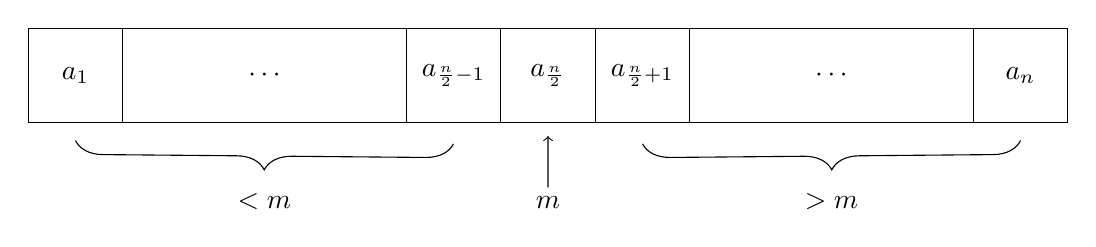
\begin{tikzpicture}[scale=1.2]

\draw (0,0) rectangle (1,1);
\node (a) at (0.5, 0.5) {$a_1$};

\draw (1,0) rectangle (4,1);
\node at (2.5, 0.5) {$\cdots$};

\draw (4,0) rectangle (5,1);
\node (b) at (4.5, 0.5) {$a_{\frac{n}{2}-1}$};

\draw (5,0) rectangle (6,1);
\node (am) at (5.5, 0.5) {$a_{\frac{n}{2}}$};

\draw (6,0) rectangle (7,1);
\node (c) at (6.5, 0.5) {$a_{\frac{n}{2}+1}$};

\draw (7,0) rectangle (10,1);
\node at (8.5, 0.5) {$\cdots$};

\draw (10,0) rectangle (11,1);
\node (d) at (10.5, 0.5) {$a_{n}$};


\node (m) at (5.5, -0.85) {$m$};
\draw[->,shorten >=0.5cm] (m) -- (am);


  \draw [decorate,decoration={brace,mirror,amplitude=10pt},xshift=-4pt,yshift=0pt] ([xshift=0cm,yshift=-.5cm]a.south) -- ([xshift=0cm,yshift=-0.5cm]b.south) node [black,midway,yshift=-0.75cm] {$< m$};

  \draw [decorate,decoration={brace,mirror,amplitude=10pt},xshift=-4pt,yshift=0pt] ([xshift=0cm,yshift=-.5cm]c.south) -- ([xshift=0cm,yshift=-0.5cm]d.south) node [black,midway,yshift=-0.75cm] {$> m$};


\end{tikzpicture}

%\caption[Array of Integers]{Array of Integers}
%\label{figure:arrayForSearching}
%\end{figure}
%
%\end{document}
%

\caption[A Sorted Array]{When an array is sorted, all elements in the left half are less than the middle element $m$, all elements in the
right half are greater than $m$.}
\label{figure:binarySearchDemo}
\end{figure}

Observe that since the array is sorted, everything in the left-half 
of the array is $< m$ and everything in the right-half of the array 
is $> m$.  We will now make one comparison between $e_k$ and $m$.
There are three cases to consider.\footnote{If duplicate elements
are in the array, then elements in the left/right half \emph{could}
be less than or equal to and greater than or equal to $m$, but this
will not affect how our algorithm works.}

\begin{enumerate}
  \item If $e_k = m$, then we've found \emph{an} element that matches
  	our key and search criteria and we are done.  We can output
	$m$ and stop the algorithm.
  \item If $e_k < m$ then we know that if a matching element exists, 
  	it must lie in the left-half of the list.  This is because all 
	elements in the right-half are $> m$.
  \item If $e_k > m$ then we know that if a matching element exists, 
  	it must lie in the right-half of the list.  This is because all 
	elements in the left-half are $< m$.
\end{enumerate}

In either of the second two cases, we have essentially cut the array
in half, halving the number of elements we need to consider.  Suppose
that the second case applies.  Then we can consider elements indexed
from $1$ to $\frac{n}{2}-1$ (we need not consider $a_{\frac{n}{2}}$ 
as the first case would have applied if we found a match).  We
can then do the same trick: check the middle element among the 
remaining elements and determine which half to cutout and which
half to consider.  We repeat this process until we've either found
the element we are looking for or the range in which we are searching
becomes ``empty'' indicating an unsuccessful search.

This description suggests a recursive solution.  Given two indices
$l, r$, we can compute the index of the middle element, $m = \frac{l + r}{2}$
and make one of two recursive calls depending on the cases identified
above.  Of course, we will need to make sure that our base case is taken
care of: if the two indices are \emph{invalid}, that is if the left
is greater than the right, $l > r$, then we know that the search
was unsuccessful.

\begin{algorithm}[H]
  \Input{A \emph{sorted} collection of elements $A = \{a_1, \ldots, a_n\}$, 
         bounds $1 \leq l, r \leq n$, and a key $e_k$}
  \Output{An element $a \in A$ such that $a = e_k$ according to some criteria; 
          $\phi$ if no such element exists}
  \If{$l > r$}{
    output $\phi$ \;
  }
  $m \leftarrow \lfloor \frac{l + r}{2} \rfloor$ \;
  \uIf{$a_m = e_k$}{ 
    output $a_m$ \;
  }
  \uElseIf{$a_m < e_k$}{ 
    \textsc{BinarySearch}$(A, m+1, r, e_k)$ \;
  }
  \Else{
    \textsc{BinarySearch}$(A, l, m-1, e_k)$ \;
  }
\caption{Recursive Binary Search Algorithm, $\textsc{BinarySearch}(A, l, r, e_k)$}
\label{algo:binarySearchRecursive}
\end{algorithm}

As discussed in Chapter \ref{chapter:recursion}, non-recursive solutions
are generally better than recursive ones.  We can design a straightforward
iterative version of binary search using a while loop.  We initialize two
index variables, $l, r$ and update them on each iteration depending on the
three cases above.  The loop stops when we've found our element or $l > r$
resulting in an unsuccessful search.  The iterative version is presented
in Algorithm \ref{algo:binarySearchIterative}, an example run of the
algorithm is shown in Figure \ref{figure:binarySearchExample}.

\begin{algorithm}[H]
  \Input{A \emph{sorted} collection of elements $A = \{a_1, \ldots, a_n\}$ 
         and a key $e_k$}
  \Output{An element $a \in A$ such that $a = e_k$ according to some criteria; 
          $\phi$ if no such element exists}
  $l \leftarrow 1$ \;
  $r \leftarrow n$ \;
  \While{$l \leq r$}{
    $m \leftarrow \lfloor \frac{l + r}{2} \rfloor$ \;
    \uIf{$a_m = e_k$}{ \label{algo:binarySearch:elemOp1}
      output $a_m$ \;
    }
    \uElseIf{$a_m < e_k$}{ \label{algo:binarySearch:elemOp2}
      $l \leftarrow (m+1)$ \;
    }
    \Else{
      $r \leftarrow (m-1)$ \;
    }
  }
  output $\phi$ \;
\caption{Iterative Binary Search Algorithm, $\textsc{BinarySearch}(A, e_k)$}
\label{algo:binarySearchIterative}
\end{algorithm}

%\documentclass[12pt]{scrbook}
%
%\usepackage{tikz}
%\usepackage{minted}
%\usetikzlibrary{decorations.pathreplacing}
%
%\usetikzlibrary{patterns}
%
%\usepackage{fullpage}
%\usepackage{subfigure}
%\begin{document}
%
%
%Lorem Ipsum is simply dummy text of the printing and typesetting industry. Lorem Ipsum has been the industry's standard dummy text ever since the 1500s, when an unknown printer took a galley of type and scrambled it to make a type specimen book. It has survived not only five centuries, but also the leap into electronic typesetting, remaining essentially unchanged. It was popularised in the 1960s with the release of Letraset sheets containing Lorem Ipsum passages, and more recently with desktop publishing software like Aldus PageMaker including versions of Lorem Ipsum.
%

\begin{figure}
\centering

\subfigure[Initially, $l = 0, r = 10$ and so we examine the middle
element at index $m = 5$ which is 12.]{

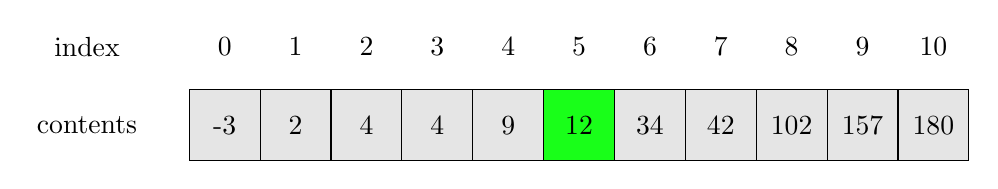
\begin{tikzpicture}
% size of each node
\def\sz{9mm}
% node style definition
\tikzstyle{block} = [
	draw, fill=black!10, rectangle,
	minimum height=\sz, minimum width=\sz ];
\tikzstyle{plain} = [draw=none,fill=none];
% array element definition
\def\arr{0, 2, 4, 4, 9, 12, 34, 42, 102};
%\def\x{0}; % x pos of arr
%\def\y{0}; % y pos of arr
%\newcounter{ind};
%\setcounter{ind}{0};
\node[plain] at (-1.75, 1) { index };
\node[plain] at (-1.75, 0) { contents };

\node[block] at (0,0) { -3 };
\node[plain] at (0,1.0) { 0 };

\node[block] at (1*\sz,0) { 2 };
\node[plain] at (1*\sz,1.0) { 1 };

\node[block] at (2*\sz,0) { 4 };
\node[plain] at (2*\sz,1.0) { 2 };

\node[block] at (3*\sz,0) { 4 };
\node[plain] at (3*\sz,1.0) { 3 };

\node[block] at (4*\sz,0) { 9 };
\node[plain] at (4*\sz,1.0) { 4 };

\node[block,fill=white!10!green] at (5*\sz,0) { 12 };
\node[plain] at (5*\sz,1.0) { 5 };

\node[block] at (6*\sz,0) { 34 };
\node[plain] at (6*\sz,1.0) { 6 };

\node[block] at (7*\sz,0) { 42 };
\node[plain] at (7*\sz,1.0) { 7 };

\node[block] at (8*\sz,0) { 102 };
\node[plain] at (8*\sz,1.0) { 8 };

\node[block] at (9*\sz,0) { 157 };
\node[plain] at (9*\sz,1.0) { 9 };

\node[block] at (10*\sz,0) { 180 };
\node[plain] at (10*\sz,1.0) { 10 };


%\foreach \item in \arr
%{
%	\node[block] (a\theind) at (\theind*\sz,0) { \item };
%	\node[plain] at (\theind*\sz,1.0) { \theind };
%	\addtocounter{ind}{1};
%}
\end{tikzpicture}

}

\subfigure[Since $64 > 12$, we update our left index variable
$l$ to $m + 1$, thus $l = 6$ and we've eliminated the left half
of the list from consideration.]{

\begin{tikzpicture}
% size of each node
\def\sz{9mm}
% node style definition
\tikzstyle{block} = [
	draw, fill=black!10, rectangle,
	minimum height=\sz, minimum width=\sz ];
\tikzstyle{plain} = [draw=none,fill=none];
% array element definition
\def\arr{0, 2, 4, 4, 9, 12, 34, 42, 102};
%\def\x{0}; % x pos of arr
%\def\y{0}; % y pos of arr
%\newcounter{ind};
%\setcounter{ind}{0};
\node[plain] at (-1.75, 1) { index };
\node[plain] at (-1.75, 0) { contents };

\node[block,pattern=north west lines, pattern color=blue] at (0,0) { -3 };
\node[plain] at (0,1.0) { 0 };

\node[block,pattern=north west lines, pattern color=blue] at (1*\sz,0) { 2 };
\node[plain] at (1*\sz,1.0) { 1 };

\node[block,pattern=north west lines, pattern color=blue] at (2*\sz,0) { 4 };
\node[plain] at (2*\sz,1.0) { 2 };

\node[block,pattern=north west lines, pattern color=blue] at (3*\sz,0) { 4 };
\node[plain] at (3*\sz,1.0) { 3 };

\node[block,pattern=north west lines, pattern color=blue] at (4*\sz,0) { 9 };
\node[plain] at (4*\sz,1.0) { 4 };

\node[block,fill=white!10!green] at (5*\sz,0) { 12 };
\node[plain] at (5*\sz,1.0) { 5 };

\node[block] at (6*\sz,0) { 34 };
\node[plain] at (6*\sz,1.0) { 6 };

\node[block] at (7*\sz,0) { 42 };
\node[plain] at (7*\sz,1.0) { 7 };

\node[block] at (8*\sz,0) { 102 };
\node[plain] at (8*\sz,1.0) { 8 };

\node[block] at (9*\sz,0) { 157 };
\node[plain] at (9*\sz,1.0) { 9 };

\node[block] at (10*\sz,0) { 180 };
\node[plain] at (10*\sz,1.0) { 10 };




%\foreach \item in \arr
%{
%	\node[block] (a\theind) at (\theind*\sz,0) { \item };
%	\node[plain] at (\theind*\sz,1.0) { \theind };
%	\addtocounter{ind}{1};
%}
\end{tikzpicture}

}



\subfigure[Our new middle index is $m = \frac{l+r}{2} = \frac{6+10}{2} = 8$, 
corresponding to the element 102.]{

\begin{tikzpicture}
% size of each node
\def\sz{9mm}
% node style definition
\tikzstyle{block} = [
	draw, fill=black!10, rectangle,
	minimum height=\sz, minimum width=\sz ];
\tikzstyle{plain} = [draw=none,fill=none];
% array element definition
\def\arr{0, 2, 4, 4, 9, 12, 34, 42, 102};
%\def\x{0}; % x pos of arr
%\def\y{0}; % y pos of arr
%\newcounter{ind};
%\setcounter{ind}{0};
\node[plain] at (-1.75, 1) { index };
\node[plain] at (-1.75, 0) { contents };

\node[block,pattern=north west lines, pattern color=blue] at (0,0) { -3 };
\node[plain] at (0,1.0) { 0 };

\node[block,pattern=north west lines, pattern color=blue] at (1*\sz,0) { 2 };
\node[plain] at (1*\sz,1.0) { 1 };

\node[block,pattern=north west lines, pattern color=blue] at (2*\sz,0) { 4 };
\node[plain] at (2*\sz,1.0) { 2 };

\node[block,pattern=north west lines, pattern color=blue] at (3*\sz,0) { 4 };
\node[plain] at (3*\sz,1.0) { 3 };

\node[block,pattern=north west lines, pattern color=blue] at (4*\sz,0) { 9 };
\node[plain] at (4*\sz,1.0) { 4 };

\node[block,pattern=north west lines, pattern color=blue] at (5*\sz,0) { 12 };
\node[plain] at (5*\sz,1.0) { 5 };

\node[block] at (6*\sz,0) { 34 };
\node[plain] at (6*\sz,1.0) { 6 };

\node[block] at (7*\sz,0) { 42 };
\node[plain] at (7*\sz,1.0) { 7 };

\node[block,fill=white!10!green] at (8*\sz,0) { 102 };
\node[plain] at (8*\sz,1.0) { 8 };

\node[block] at (9*\sz,0) { 157 };
\node[plain] at (9*\sz,1.0) { 9 };

\node[block] at (10*\sz,0) { 180 };
\node[plain] at (10*\sz,1.0) { 10 };




%\foreach \item in \arr
%{
%	\node[block] (a\theind) at (\theind*\sz,0) { \item };
%	\node[plain] at (\theind*\sz,1.0) { \theind };
%	\addtocounter{ind}{1};
%}
\end{tikzpicture}

}

\subfigure[Since $64 < 102$, we update the right index variable 
$r$ to $m - 1 = 7$, eliminating the right half of the subarray.]{

\begin{tikzpicture}
% size of each node
\def\sz{9mm}
% node style definition
\tikzstyle{block} = [
	draw, fill=black!10, rectangle,
	minimum height=\sz, minimum width=\sz ];
\tikzstyle{plain} = [draw=none,fill=none];
% array element definition
\def\arr{0, 2, 4, 4, 9, 12, 34, 42, 102};
%\def\x{0}; % x pos of arr
%\def\y{0}; % y pos of arr
%\newcounter{ind};
%\setcounter{ind}{0};
\node[plain] at (-1.75, 1) { index };
\node[plain] at (-1.75, 0) { contents };

\node[block,pattern=north west lines, pattern color=blue] at (0,0) { -3 };
\node[plain] at (0,1.0) { 0 };

\node[block,pattern=north west lines, pattern color=blue] at (1*\sz,0) { 2 };
\node[plain] at (1*\sz,1.0) { 1 };

\node[block,pattern=north west lines, pattern color=blue] at (2*\sz,0) { 4 };
\node[plain] at (2*\sz,1.0) { 2 };

\node[block,pattern=north west lines, pattern color=blue] at (3*\sz,0) { 4 };
\node[plain] at (3*\sz,1.0) { 3 };

\node[block,pattern=north west lines, pattern color=blue] at (4*\sz,0) { 9 };
\node[plain] at (4*\sz,1.0) { 4 };

\node[block,pattern=north west lines, pattern color=blue] at (5*\sz,0) { 12 };
\node[plain] at (5*\sz,1.0) { 5 };

\node[block] at (6*\sz,0) { 34 };
\node[plain] at (6*\sz,1.0) { 6 };

\node[block] at (7*\sz,0) { 42 };
\node[plain] at (7*\sz,1.0) { 7 };

\node[block,fill=white!10!green] at (8*\sz,0) { 102 };
\node[plain] at (8*\sz,1.0) { 8 };

\node[block,pattern=north west lines, pattern color=blue] at (9*\sz,0) { 157 };
\node[plain] at (9*\sz,1.0) { 9 };

\node[block,pattern=north west lines, pattern color=blue] at (10*\sz,0) { 180 };
\node[plain] at (10*\sz,1.0) { 10 };




%\foreach \item in \arr
%{
%	\node[block] (a\theind) at (\theind*\sz,0) { \item };
%	\node[plain] at (\theind*\sz,1.0) { \theind };
%	\addtocounter{ind}{1};
%}
\end{tikzpicture}

}


\subfigure[Here, $l = 6, r = 7$, and so our new middle index is
$m = \lfloor \frac{6 + 7}{2}\rfloor = 6$.  Since $64 > 34$, we 
update our left index variable $l$ to $m+1 = 7$]{

\begin{tikzpicture}
% size of each node
\def\sz{9mm}
% node style definition
\tikzstyle{block} = [
	draw, fill=black!10, rectangle,
	minimum height=\sz, minimum width=\sz ];
\tikzstyle{plain} = [draw=none,fill=none];
% array element definition
\def\arr{0, 2, 4, 4, 9, 12, 34, 42, 102};
%\def\x{0}; % x pos of arr
%\def\y{0}; % y pos of arr
%\newcounter{ind};
%\setcounter{ind}{0};
\node[plain] at (-1.75, 1) { index };
\node[plain] at (-1.75, 0) { contents };

\node[block,pattern=north west lines, pattern color=blue] at (0,0) { -3 };
\node[plain] at (0,1.0) { 0 };

\node[block,pattern=north west lines, pattern color=blue] at (1*\sz,0) { 2 };
\node[plain] at (1*\sz,1.0) { 1 };

\node[block,pattern=north west lines, pattern color=blue] at (2*\sz,0) { 4 };
\node[plain] at (2*\sz,1.0) { 2 };

\node[block,pattern=north west lines, pattern color=blue] at (3*\sz,0) { 4 };
\node[plain] at (3*\sz,1.0) { 3 };

\node[block,pattern=north west lines, pattern color=blue] at (4*\sz,0) { 9 };
\node[plain] at (4*\sz,1.0) { 4 };

\node[block,pattern=north west lines, pattern color=blue] at (5*\sz,0) { 12 };
\node[plain] at (5*\sz,1.0) { 5 };

\node[block,fill=white!10!green] at (6*\sz,0) { 34 };
\node[plain] at (6*\sz,1.0) { 6 };

\node[block] at (7*\sz,0) { 42 };
\node[plain] at (7*\sz,1.0) { 7 };

\node[block,pattern=north west lines, pattern color=blue] at (8*\sz,0) { 102 };
\node[plain] at (8*\sz,1.0) { 8 };

\node[block,pattern=north west lines, pattern color=blue] at (9*\sz,0) { 157 };
\node[plain] at (9*\sz,1.0) { 9 };

\node[block,pattern=north west lines, pattern color=blue] at (10*\sz,0) { 180 };
\node[plain] at (10*\sz,1.0) { 10 };




%\foreach \item in \arr
%{
%	\node[block] (a\theind) at (\theind*\sz,0) { \item };
%	\node[plain] at (\theind*\sz,1.0) { \theind };
%	\addtocounter{ind}{1};
%}
\end{tikzpicture}

}

\subfigure[Since $64 > 42$ we again update our left index variable $l$
to $m + 1 = 8$.]{

\begin{tikzpicture}
% size of each node
\def\sz{9mm}
% node style definition
\tikzstyle{block} = [
	draw, fill=black!10, rectangle,
	minimum height=\sz, minimum width=\sz ];
\tikzstyle{plain} = [draw=none,fill=none];
% array element definition
\def\arr{0, 2, 4, 4, 9, 12, 34, 42, 102};
%\def\x{0}; % x pos of arr
%\def\y{0}; % y pos of arr
%\newcounter{ind};
%\setcounter{ind}{0};
\node[plain] at (-1.75, 1) { index };
\node[plain] at (-1.75, 0) { contents };

\node[block,pattern=north west lines, pattern color=blue] at (0,0) { -3 };
\node[plain] at (0,1.0) { 0 };

\node[block,pattern=north west lines, pattern color=blue] at (1*\sz,0) { 2 };
\node[plain] at (1*\sz,1.0) { 1 };

\node[block,pattern=north west lines, pattern color=blue] at (2*\sz,0) { 4 };
\node[plain] at (2*\sz,1.0) { 2 };

\node[block,pattern=north west lines, pattern color=blue] at (3*\sz,0) { 4 };
\node[plain] at (3*\sz,1.0) { 3 };

\node[block,pattern=north west lines, pattern color=blue] at (4*\sz,0) { 9 };
\node[plain] at (4*\sz,1.0) { 4 };

\node[block,pattern=north west lines, pattern color=blue] at (5*\sz,0) { 12 };
\node[plain] at (5*\sz,1.0) { 5 };

\node[block,pattern=north west lines, pattern color=blue] at (6*\sz,0) { 34 };
\node[plain] at (6*\sz,1.0) { 6 };

\node[block,fill=white!10!green] at (7*\sz,0) { 42 };
\node[plain] at (7*\sz,1.0) { 7 };

\node[block,pattern=north west lines, pattern color=blue] at (8*\sz,0) { 102 };
\node[plain] at (8*\sz,1.0) { 8 };

\node[block,pattern=north west lines, pattern color=blue] at (9*\sz,0) { 157 };
\node[plain] at (9*\sz,1.0) { 9 };

\node[block,pattern=north west lines, pattern color=blue] at (10*\sz,0) { 180 };
\node[plain] at (10*\sz,1.0) { 10 };




%\foreach \item in \arr
%{
%	\node[block] (a\theind) at (\theind*\sz,0) { \item };
%	\node[plain] at (\theind*\sz,1.0) { \theind };
%	\addtocounter{ind}{1};
%}
\end{tikzpicture}

}

\subfigure[Since $l = 8$ and $r = 7$, $l > r$ and the loop terminates, 
resulting in an unsuccessful search.]{

\begin{tikzpicture}
% size of each node
\def\sz{9mm}
% node style definition
\tikzstyle{block} = [
	draw, fill=black!10, rectangle,
	minimum height=\sz, minimum width=\sz ];
\tikzstyle{plain} = [draw=none,fill=none];
% array element definition
\def\arr{0, 2, 4, 4, 9, 12, 34, 42, 102};
%\def\x{0}; % x pos of arr
%\def\y{0}; % y pos of arr
%\newcounter{ind};
%\setcounter{ind}{0};
\node[plain] at (-1.75, 1) { index };
\node[plain] at (-1.75, 0) { contents };

\node[block,pattern=north west lines, pattern color=blue] at (0,0) { -3 };
\node[plain] at (0,1.0) { 0 };

\node[block,pattern=north west lines, pattern color=blue] at (1*\sz,0) { 2 };
\node[plain] at (1*\sz,1.0) { 1 };

\node[block,pattern=north west lines, pattern color=blue] at (2*\sz,0) { 4 };
\node[plain] at (2*\sz,1.0) { 2 };

\node[block,pattern=north west lines, pattern color=blue] at (3*\sz,0) { 4 };
\node[plain] at (3*\sz,1.0) { 3 };

\node[block,pattern=north west lines, pattern color=blue] at (4*\sz,0) { 9 };
\node[plain] at (4*\sz,1.0) { 4 };

\node[block,pattern=north west lines, pattern color=blue] at (5*\sz,0) { 12 };
\node[plain] at (5*\sz,1.0) { 5 };

\node[block,pattern=north west lines, pattern color=blue] at (6*\sz,0) { 34 };
\node[plain] at (6*\sz,1.0) { 6 };

\node[block,pattern=north west lines, pattern color=blue] at (7*\sz,0) { 42 };
\node[plain] at (7*\sz,1.0) { 7 };

\node[block,pattern=north west lines, pattern color=blue] at (8*\sz,0) { 102 };
\node[plain] at (8*\sz,1.0) { 8 };

\node[block,pattern=north west lines, pattern color=blue] at (9*\sz,0) { 157 };
\node[plain] at (9*\sz,1.0) { 9 };

\node[block,pattern=north west lines, pattern color=blue] at (10*\sz,0) { 180 };
\node[plain] at (10*\sz,1.0) { 10 };




%\foreach \item in \arr
%{
%	\node[block] (a\theind) at (\theind*\sz,0) { \item };
%	\node[plain] at (\theind*\sz,1.0) { \theind };
%	\addtocounter{ind}{1};
%}
\end{tikzpicture}

}

\caption[Binary Search Example 1]{The worst case scenario for binary search, 
resulting in an unsuccessful search.  This example is run on a 0-indexed array
with an array of integers of size 11.}
\label{figure:binarySearchExample}

\end{figure}




%\end{document}


\subsection{Analysis}

When algorithms are implemented and run on a computer, they require a
certain amount of \emph{resources}.  In general, we could consider a lot
of different resources such as computation time and memory.  Algorithm
analysis involves quantifying how many resource(s) an algorithm requires
to execute with respect to the size of the input it is run on.

When analyzing algorithms, we want to keep the analysis as abstract and 
general as possible independent of any particular language, framework or
hardware.  We could always update the hardware on which we run our implementation, 
but that does not necessarily make the \emph{algorithm} faster, it only means
that more \emph{steps} of the algorithm can be run in less time.  The
number of operations that the algorithm performs remains the same.  In
fact, the concept of an algorithm itself is a mathematical concept that
predates modern computers by thousands of years.  One of the oldest algorithms,
for example, Euler's GCD (greatest common divisor) algorithm dates to 300
BCE.  Whether or not you're ``running'' it on a piece of papyrus 2,300 years
ago or on a modern supercomputer, the same number of divisions and subtractions
are performed.

To keep things abstract, we analyze an algorithm using pseudocode and identify
an \emph{elementary operation}.  This is generally the most common or most
``expensive'' operation that the algorithm performs.  Sometimes there may be more
than one reasonable choice for an elementary operation which may give different
analysis results.  However, we generally do \emph{not} consider basic operations
that are necessary to the \emph{control flow} of an algorithm.  For example, 
variable assignments or the iteration of index variables.

Once we have identified an elementary operation, we can quantify the complexity
of an algorithm by analyzing the number of times the elementary operation is
executed with respect to the \emph{input size}.  For a collection, the input
size is generally the number of elements in the collection, $n$.  We can
then characterize the number of elementary operations and thus the complexity
of the algorithm itself as a \emph{function} of the input size.  We illustrate
this process by analyzing and comparing the two search algorithms.

\subsubsection{Linear Search Analysis}

When considering the linear search algorithm, the input size is clearly the
number of elements in the collection, $n$.  The best candidate for the
elementary operation is the comparison (Line \ref{algo:linearSearch:elemOp}, 
Algorithm \ref{algo:linearSearch}).  To analyze this algorithm, we need
to determine how many comparisons are made with respect to the size of
the collection, $n$.

As we saw in the examples, the number of comparisons made by linear search
can vary depending on the element we're searching and the configuration of
the collection being searched.  Because of this variability, we can 
analyze the algorithm in one of three ways: by looking at the best case
scenario, worst case scenario, and average case scenario.

The best case scenario is when the number of operations is \emph{minimized}.
For linear search, the best case scenario happens when we get lucky and
the first element that we examine matches our criteria, requiring only a 
single comparison operation.  In general, it is not reasonable to assume
that the best case scenario will be commonly encountered.

The worst case scenario is when the number of operations is \emph{maximized}.
This happens when we get ``unlucky'' and have to search the entire collection
finding a match at the last element or not finding a match at all.  In either
case, we make $n$ comparisons to search the collection.

A formal average case analysis is not difficult, but is a bit beyond the
scope of the present analysis.  However, informally, we could expect to make
about $\frac{n}{2}$ comparisons for successful searches if we assume that
all elements have a uniform probability of being searched for.

Both the worst-case and average-case are reasonable scenarios from which to
analyze the linear search algorithm.  In the end, however, the only difference
between the two analyses is a constant factor.  Both analyses result in two
linear functions, 
  $$f_1(n) = n \quad f_2(n) = \frac{1}{2}n$$
The only difference being the constant factor $\frac{1}{2}$.  In fact, this
is why the algorithm is called \emph{linear} search.  The number of comparison
operations performed by the algorithm \emph{grows} linearly with respect
to the input size.  For example, if we were to double the input size from
$n$ to $2n$, then we would expect the number of comparisons to search the
collection would also double (this applies in either the worst-case or average-case
scenarios).  This is what is most important in algorithm analysis: quantifying
the complexity of an algorithm by the rate of growth of the operations (and
thus resources) required to execute the algorithm as the input size $n$ 
grows.\footnote{In fact, this is the basis of Big-O analysis, something that 
we will not discuss in detail here, but is of prime importance when analyzing
algorithms.}

\subsubsection{Binary Search Analysis}

Like linear search, the input size is the size of the collection $n$ and the
elementary operation is the comparison.  As presented in the pseudocode, 
binary search would seem to perform \emph{two} comparisons (Lines
\ref{algo:binarySearch:elemOp1} and \ref{algo:binarySearch:elemOp1} in Algorithm
\ref{algo:binarySearchIterative}).  However, to make the analysis simpler, we
will instead count one comparison operation per iteration of the 
while loop.  This is a reasonable simplification; in practice the comparison
operation would likely involve a single function call, after which 
distinguishing between the three cases is a simple matter of control flow.
Further, even if we were to consider both operations, it would only contribute
a constant factor of 2 to the final analysis.

Since we perform one comparison for each iteration of the while loop, we need
to determine how many times the while loop executes.  In the worst case, the
number of iterations is maximized when we fail to find an element that does
not match our criteria.  However each iteration essentially cuts the array in
half each time.  That is, if we start with an array of size $n$, then after the 
first iteration, it is of size $\frac{n}{2}$.  After the second iteration
we have cut it in half again, so it is of size $\frac{n}{4}$, after the third
iteration it is of size $\frac{n}{8}$ and so on.  More generally, after
$k$ iterations, the size of the array is
  $$\frac{n}{2^k}$$
The loop terminates one iteration \emph{after} the the index variables are 
equal, $l = r$.  Equivalently, when $l = r$, the size of the subarray under consideration is 1.  That is, the algorithm stops when the array size has
been cut down to 1:
  $$\frac{n}{2^k} = 1$$
Solving for $k$ gives us the number of iterations:
  $$k = \log_2{(n)}$$
That is, binary search performs a logarithmic number of comparisons in the worst
case.  As we will see, this is \emph{exponentially} better than linear search.

{\renewcommand{\arraystretch}{1.5}
\begin{table}[h]
\centering
\begin{tabular}{c|c|c}
Iteration & Array Size & Comparisons \\
\hline\hline
1 & $\frac{n}{2}$ & 1 \\
2 & $\frac{n}{4}$ & 1 \\
3 & $\frac{n}{8}$ & 1 \\
4 & $\frac{n}{16}$ & 1 \\
\vdots & \vdots & \vdots \\
$k$ & $\frac{n}{2^k}$ & 1 \\
\vdots & \vdots & \vdots \\
$\log_2{(n)}$ & 1 & 1 \\
$\log_2{(n)}+1$ & 0 & 1 \\
\hline
\multicolumn{2}{c|}{Total} & $\log_2{(n)} + 1$ \\
\end{tabular}
\caption{Number of comparisons and array size during the execution of binary search.}
\label{table:binarySearchComparisons}
\end{table}
}

\subsubsection{Comparative Analysis}

Binary search presents a clear advantage over linear search.  There is
an \emph{exponential} difference between a linear function, $\frac{n}{2}$
and a logarithmic function, $\log_2{(n)}$.

To put this in
perspective, consider searching a \emph{moderately} large database of 1
trillion ($10^{12}$) records.\footnote{In the era of ``big data'', 1 trillion
records only qualifies as \emph{moderately} large.}  Using linear search, 
even in the average-case scenario would require about
  $$\frac{10^{12}}{2} = 5 \times 10^11$$
or about 500 billion comparisons.  However, using binary search would only
require at most 
  $$\log_2{(10^{12})} = 12 \cdot \log_2{(10)} < 40$$ 
comparisons to search.  This is a \emph{huge} difference in performance.

As another comparison, let's consider how each algorithm's complexity
grows as we increase the size of the collection being searched.  As observed
earlier, if we double the input size, $n \rightarrow 2n$, we would expect
the number of comparisons performed by linear search to also double.
However, if we double the input size for binary search, we get the following.
  $$\log_2{(2n)} = \log_2{(2)} + \log{(n)} = \log{(n)} + 1$$
That is, only a single additional comparison is necessary to search an array
of twice the size.

The difference between these two algorithms shows up in many different instances.
Figure \ref{figure:windows7Example} contains a screen shot of the search feature
in Windows 7.  When searching for particular files or content in particular files,
the search can be greatly increased if the files have been \emph{indexed}, that
is, sorted.  As the dialog indicates, non-indexed (unsorted) records will take
far longer to search.

\begin{figure}[h]
\centering
\includegraphics[scale=0.5]{images/windows7Example}
\caption{Illustrative example of the benefit of ordered (indexed) elements, Windows 7}
\label{figure:windows7Example}
\end{figure}

Though binary search presents a clear advantage over linear search, it only works
if the collection has been sorted.\footnote{Binary search also only works when
searching an array with random access to its elements.  The performance of binary
search cannot generally be realized with data structures such as linked lists or 
unordered sets.}  Thus, we now turn our attention to the problem of sorting
a collection.

\section{Sorting}

Sorting a collection of data is another fundamental data operation.  It is
conceptually simple, but is ubiquitous.  There are a large variety of
algorithms, data structures and applications built around the problem
of sorting.  As we've already seen, being able to sort a collection provides 
a huge speed up when searching for a particular element.  Sorting provides 
a natural way to store and organize data.  

\begin{problem}[Sorting]
~\\
\textbf{Given:} a collection of \emph{orderable} elements, $A =\{a_1, a_2, \ldots, a_n\}$\\
\textbf{Output:} A permuted list of elements $A' = \{a_1', a_2', \ldots, a_n'\}$ according to a specified order
\end{problem}

The requirement that the collection be made of ``orderable'' elements can be
a bit technical\footnote{We require that $A$ be a \emph{total order}, a 
partially ordered binary relation such that all pairs are comparable.}, but essentially 
we need to be guaranteed that given two elements, $a, b$ in the collection, 
we can determine whether $a < b$, $a = b$ or $a > b$.  If such a determination
cannot be made, then sorting is impossible.

Again, we can consider variations on this problem.  We may want our collection
to be sorted in ascending or descending order.\footnote{Technically, these are
referred to as \emph{non-decreasing} and \emph{non-increasing} respectively.  
This is because the collection could contain duplicate elements and not lead
to a strictly increasing or strictly decreasing ordering.} We may also want
the collection itself to be \emph{permuted} (that is, reordered) or we may
instead want a \emph{copy} of the collection to be created and sorted so that
the original is unchanged.

We will examine several standard sorting algorithms (though there are dozens
of algorithms, we will only focus on a few of the more common ones).  As with 
searching, we can analyze a sorting algorithm based on the number of 
comparisons it makes in the worst, best, or average cases.  We may also look
at alternative resources or operations: how many swaps does the algorithm make?
How much extra memory is required?  Etc.

Though we will examine, analyze and compare several sorting algorithms, most
programming languages provide standard functionality to sort a collection of
elements.  It is generally preferable to use the functionality built into 
whatever language you're using rather that reimplementing your own.  Typically, 
these functions are well-designed, well-tested, optimized and more efficient
than any custom alternatives.

\subsection{Selection Sort}

TODO: HERE

\begin{itemize}
  \item Iterate through the elements in the list and find the minimal element in the list
  \item Swap the minimal element with the ``first'' element
  \item Repeat the process on the remaining $n-1$ elements
  \item Pseudocode presented in Algorithm \ref{algo:selectionSort}
  \item Java code (for integers) presented in Code Sample \ref{code:javaSelectionSort}
  \item C code (for integers) presented in Code Sample \ref{code:cSelectionSort}
  \item Example
  \item Note: Selection sort is not stable, an example: $2_a, 2_b, 1, 5$; the first swap would result in $1, 2_b, 2_a, 5$ and no subsequent changes would be made.
\end{itemize}

\subsubsection{Pseudocode}

    \begin{algorithm}[H]
     \Input{A collection $A = \{a_1, \ldots, a_n\}$}
     \Output{An array $A'$ containing all elements of $A$ in nondecreasing order}
     \For{$i = 1, \ldots, (n-1)$}{
       $a_{min} \leftarrow a_i$ \;
       \For{$j = (i+1), \ldots, n$}{
         \If{$a_{min} > a_j$}{
           $min \leftarrow a_j$ \;
         }
       }
       swap $a_{min}$ and $a_i$ \;
     }
    \caption{Selection Sort}
    \label{algo:selectionSort}
    \end{algorithm}

\subsubsection{Analysis}

\begin{itemize}
  \item Comparison performed: once, inner loop, outer loop
  \item In total:
    $$\sum_{i=1}^{n-1} \sum_{j=(i+1)}^{n} 1 = \sum_{i=1}^{n-1} (n - i) = n(n-1) - \sum_{i=1}^{n-1} i =  n(n-1) - \frac{n(n-1)}{2} =  \frac{n(n-1)}{2}$$
  \item Selection Sort is $O(n^2)$
\end{itemize}

\subsection{Insertion Sort}

\begin{itemize}
  \item If we consider just the first element, the list is \emph{sorted}
  \item Now consider the second element: we can \emph{insert} it in the currently sorted sublist
  \item In general: at the $k$-th iteration, assume that elements $a_1, \ldots, a_k$ are sorted
  \item Insert element $a_{k+1}$ into the proper location among elements $a_1, \ldots, a_k$
  \item Insertion is performed by \emph{shifting} $a_{k+1}$ down until its in the right spot
  \item Pseudocode presented in Algorithm \ref{algo:insertionSort}
  \item Java code (for integers) presented in Code Sample \ref{code:javaInsertionSort}
  \item C code (for integers) presented in Code Sample \ref{code:cInsertionSort}
  \item Example
\end{itemize}

\subsubsection{Pseudocode}

    \begin{algorithm}[H]
     \Input{A collection $A = \{a_1, \ldots, a_n\}$}
     \Output{An array $A'$ containing all elements of $A$ in nondecreasing order}
     \For{$i = 2, \ldots, n$}{
       $x \leftarrow a_i$ \;
       $j \leftarrow i$ \;
       \While{$j > 1$ and $a_{j-1} > x$}{
         $a_j \leftarrow a_{j-1}$ \;
         decrement $j$ \;
       }
       $a_j \leftarrow x$ \;
     }
    \caption{Insertion Sort}
    \label{algo:insertionSort}
    \end{algorithm}

\subsubsection{Analysis}

\begin{itemize}
  \item Best case: list is already sorted, number of comparisons is $(n-1)$
  \item Worst case: reversed list; each iteration shifts the element all the way down
  \item First iteration: 1 comparison, 2nd: at most 2, etc., last iteration: at most $(n-1)$ comparisons
	$$\sum_{i=1}^{n-1} i = \frac{n(n-1)}{2}$$
  \item Worst case: $O(n^2)$
  \item A more complex analysis for the \emph{average case}, but still $O(n^2)$
  \item Practical consideration: insertion sort is inherently adaptive; good performance in practice
  \item Very efficient on small lists, especially if there is already some structure (partially ordered) to them
\end{itemize}


\subsection{Quick Sort}

Due to Tony Hoare in the early 1960s \cite{Hoare:1961:AQ:366622.366644,Quicksort}


\begin{itemize}
  \item Choose a \emph{pivot} element $a_p$
  \item Partition all other elements \emph{around} this pivot: move all less elements to the ``left'' side of the list; all greater elements to the ``right''
  \item Place pivot element between them
  \item Repeat the process on the two partitions until each sublist is trivially sorted (empty or a single element)
  \item Pseudocode presented in Algorithm \ref{algo:quickSort} and \ref{algo:partition}
  \item Java code (for integers) presented in Code Sample \ref{code:javaQuickSort}
  \item C code (for integers) presented in Code Sample \ref{code:cQuickSort}
  \item Example
\end{itemize}

\subsubsection{Pseudocode}

    \begin{algorithm}[H]
     \Input{A collection $A = \{a_1, \ldots, a_n\}$, indices $l, r$}
     \Output{An array $A'$ containing all elements of $A$ in nondecreasing order}
      \If{$l<r$}{
        $s = $ \textsc{Partition}$(A[l\ldots r])$ \;
        \textsc{QuickSort}$(A[l\ldots (s-1)])$ \;
        \textsc{QuickSort}$(A[(s+1) \ldots r])$ \;
      }
    \caption{Quick Sort}
    \label{algo:quickSort}
    \end{algorithm}

    \begin{algorithm}[H]
     \Input{Integer array $\mathcal{A}$, sub-indices $1 \leq l, r \leq n$}
     \Output{A \emph{partitioned} integer array $\mathcal{A}'$ such that
             all $A[l\ldots(j-1)] \leq A[j] \leq A[(j+1)\ldots r]$ and
             an index $j$ of the pivot element.}
     $pivot \leftarrow A[l]$ \; %\emph{//note the first element is arbitrarily chosen}\\
     $i \leftarrow l$ \;
     $j \leftarrow (r+1)$ \;
     \Repeat{$i \geq j$}{
       \Repeat{$a_i \geq pivot$}{
         $i \leftarrow (i+1)$ \;
         }
       \Repeat{$a_j \leq pivot$}{
         $j \leftarrow (j-1)$ \;
         }
       swap $a_i$, $a_j$ \;
       }
       swap $a_i$, $a_j$ \Comment{Undo the last swap}
       swap $a_l$, $a_j$ \Comment{Swap the pivot}
    \textbf{return} $j$ \;
    \caption{In-Place Partition}
    \label{algo:partition}
    \end{algorithm}

\subsubsection{Analysis}

\begin{itemize}
  \item Performance of quick sort is highly dependent on how the \emph{even} the partitioning is
  \item Partitioning depends on pivot choice
\end{itemize}

Best Case
\begin{itemize}
  \item Ideal pivot choice: always choose the median element
  \item Evenly divides the list into two equal parts
  \item Two calls to quick sort on lists roughly half the size
  \item A linear number of comparisons to partition
  \item Recurrence:
	$$C(n) = 2C\left(\frac{n}{2}\right) + n$$
  \item By the Master Theorem, $O(n\log{n})$
\end{itemize}

Worst Case
\begin{itemize}
  \item Worst pivot choice: an extremal element
  \item Divides into an empty list and a list of size $(n-1)$
  \item Only one recursive call is necessary, but on a list of size $(n-1)$
  \item Recurrence:
	$$C(n) = C(n-1) + n$$
  \item Back substitution yields $O(n^2)$
\end{itemize}

Average Case
\begin{itemize}
  \item Even if the list is is split by a constant proportion, still $O(n\log{n})$
  \item A careful average case analysis also yields
	$$C(n) \approx 1.38n\log{n}$$
  \item Still $O(n\log{n})$
\end{itemize}

Pivot Choice: Pivot choice greatly affects performance; several strategies:
\begin{itemize}
  \item Median-of-Three -- Among three elements choose the median.
        \begin{itemize}
         \item Guarantees that the pivot choice will never be the
               worst case.
         \item Does not guarantee $\Theta(n\log{n})$.
        \end{itemize}
  \item Random Element -- Randomly select an index for a pivot element.
        \begin{itemize}
         \item Guarantees \emph{average} running time of $\Theta(n\log{n})$.
         \item Extra work to randomly select a pivot.
        \end{itemize}
  \item Linear Time Median Finding.
        \begin{itemize}
         \item An algorithm exists that runs in $\Theta(n)$ time to
               find the median of $n$ objects.
         \item Guarantees $\Theta(n\log{n})$ in all cases.
         \item Complicated; recursive; \emph{huge} overhead.
        \end{itemize}
\end{itemize}

\subsection{Merge Sort}

Due to John von Neumann, 1945 (as reported by Knuth \cite{Knuth:1970:VNF:356580.356581}).

\begin{itemize}
  \item Divide the list into two (roughly) equal parts and recursively sort each
  \item Recursion stops when the list is trivially sorted (empty or a single element)
  \item When returning from the recursion, \emph{merge} the two lists together
  \item Since both sublists are sorted, we only need to maintain an index to each list, add the least element, etc.
  \item Only a linear amount of work to merge two sorted lists
  \item Pseudocode presented in Algorithm \ref{algo:mergeSort}
  \item Java code (for integers) presented in Code Sample \ref{code:javaMergeSort}
  \item C code (for integers) presented in Code Sample \ref{code:cMergeSort}
  \item Example
\end{itemize}

\subsubsection{Pseudocode}

    \begin{algorithm}[H]
     \Input{An array, sub-indices $1\leq l, r \leq n$}
     \Output{An array $A'$ such that $A[l, \ldots, r]$ is sorted}
     \If{$l < r$} {
        $\textsc{MergeSort}(A, l, \lfloor\frac{r+l}{2}\rfloor)$ \;
        $\textsc{MergeSort}(A, \lceil\frac{r+l}{2}\rceil, r)$ \;
        Merge sorted lists $A[l, \ldots, \lfloor\frac{r+l}{2}\rfloor]$ and$A[\lceil\frac{r+l}{2}\rceil, \ldots, r]$ \;
      }
    \caption{Merge Sort}
    \label{algo:mergeSort}
    \end{algorithm}

\subsubsection{Analysis}

\begin{itemize}
  \item Because merge sort divides the list \emph{first}, an even split is \emph{guaranteed}
  \item After the recursion, a linear amount of work is done to merge the two lists
  \item Basic idea:
	\begin{itemize}
	  \item Keep two index pointers to each sublist
	  \item Copy the minimal element, advance the pointer
	  \item Until one list is empty, then just copy the rest of the other
	\end{itemize}
  \item Requires use of $O(n)$-sized temporary array
  \item Recurrence:
	$$C(n) = 2C\left(\frac{n}{2}\right) + n$$
  \item By the Master Theorem, $O(n\log{n})$
  \item In fact, a guarantee (best, worst, average are the same)
\end{itemize}

\subsection{Heap Sort}

Due to J.\ W.\ J.\ Williams, 1964 \cite{williams1964algorithm}.

\subsection{Tim Sort}

Due to Tim Peters in 2002 \cite{Peters2002} who originally wrote it for the Python language.  It has since been adopted 
in Java (version 7 for arrays of non-primitive types).

\subsection{Summary}

To summarize, consider the properties of each sorting algorithm
as depicted in Table \ref{table:sortingSummary}.

\begin{table}[h]
\centering
\begin{tabular}{|c|c|c|c|c|p{3cm}|}
\hline
\multirow{2}{*}{Algorithm} & \multicolumn{3}{|c|}{Complexity} & \multirow{2}{*}{Stability} & \multirow{2}{*}{Notes} \\ \cline{2-4}
~ & Best & Average & Worst & ~ & ~ \\
\hline
Bubble Sort & $O(n^2)$ & $O(n^2)$ & $O(n^2)$ & Stable & \\
\hline
Selection Sort & $O(n^2)$ & $O(n^2)$ & $O(n^2)$ & Not Stable & \\
\hline
Insertion Sort & $O(n)$ & $O(n^2)$ & $O(n^2)$ & Stable & Best in practice for small collections\\
\hline
Quick Sort & $O(n\log{n})$ & $O(n\log{n})$ & $O(n^2)$ & Not Stable & Performance depends on pivot choices\\
\hline
Merge Sort & $\Theta(n\log{n})$ & $O(n\log{n})$ & $O(n\log{n})$ & Stable & Guaranteed $\Theta(n\log{n})$ \\
\hline
\end{tabular}
\caption{Summary of Sorting Algorithms}
\label{table:sortingSummary}
\end{table}

\section{Other Considerations}

\subsection{Preventing Arithmetic Errors in Binary Search}

Recall that in binary search, we need to compute the index of the middle element.
Given a left $l$ and right $r$ index variable, we computed the middle index
as 
  $$m \leftarrow \lfloor \frac{l + r}{2} \rfloor$$
Though mathematically correct, when implementing an expression like this, 
care must be taken.  We may initially translate this pseudocode into a line
that looks something like the following.
  
\mintinline{c}{int middle_index = (left + right) / 2;}

However, this is prone to arithmetic errors in certain situations, particularly
when dealing with large arrays.  If the variables \mintinline{c}{left} 
and \mintinline{c}{right} have a sum that exceeds the maximum value that 
a signed 32-bit integer can hold ($2^31 - 1 = 2,147,483,647$), then 
overflow will occur before the division by 2, leading to a (potentially) 
negative index value and thus an invalid out-of-bounds error or exception.

One solution would be to use a variable type that supports larger
values.  For example, a 64-bit signed integer would be able to handle
arrays of 9.223 quintillion elements.  However, depending on the language, 
you may not be able to use such variable types as index values.

Another solution is to use operations that do not introduce this 
potential for overflow.  For example, 
  $$\frac{l + r}{2} = l + \frac{(r - l)}{2}$$
but the expression on the right hand side will not be prone to overflow.  
Thus the code,

\mintinline{c}{int middle_index = left + (right - left) / 2;}

would be safer to use.  In fact, this bug is quite common 
\cite{Pattis:1988:TEB:52964.53012} and was in the Java implementation
of binary search, unreported for nearly a decade \cite{Bloch2006}.

\subsection{Avoiding the Difference Trick}

\subsection{Importance of a Total Order}

Breaking ties, sorted types

\subsection{More Gotchas}

\subsection{Sorting Stability}


Sorting stability: A sorting algorithm is said to be \emph{stable} if the relative order of ``equal'' elements is preserved.
\begin{itemize}
  \item Example: suppose that a list contains $10, 2_a, 5, 2_b$; a stable sorting algorithm would produce $2_a, 2_b, 5, 10$
	while a non-stable sorting algorithm may produce $2_b, 2_a, 5, 10$.
  \item Stable sorts are important for data presentation (sorting by two columns/categories)
  \item Stability depends on inequalities used and behavior of algorithms
\end{itemize}


